\section{Composition Approaches}
Composition approaches propose to compose models/languages into a new model/language. We categorize these approaches into approaches that compose models and approaches that compose languages, in both structural and behavioral way. In the following, we first present \emph{Model Composition Approaches}, and then, we continue with \emph{Language Composition Approaches}.
 
\subsection{Model Composition Approaches}
Model composition has as goal to get a resulting model that is built by composing one or more models of the same language or from different languages. The resulting model can conform to input model languages, or to a different language (see Figure~\ref{fig:modelcompo}).

\begin{figure}
	\begin{center}
		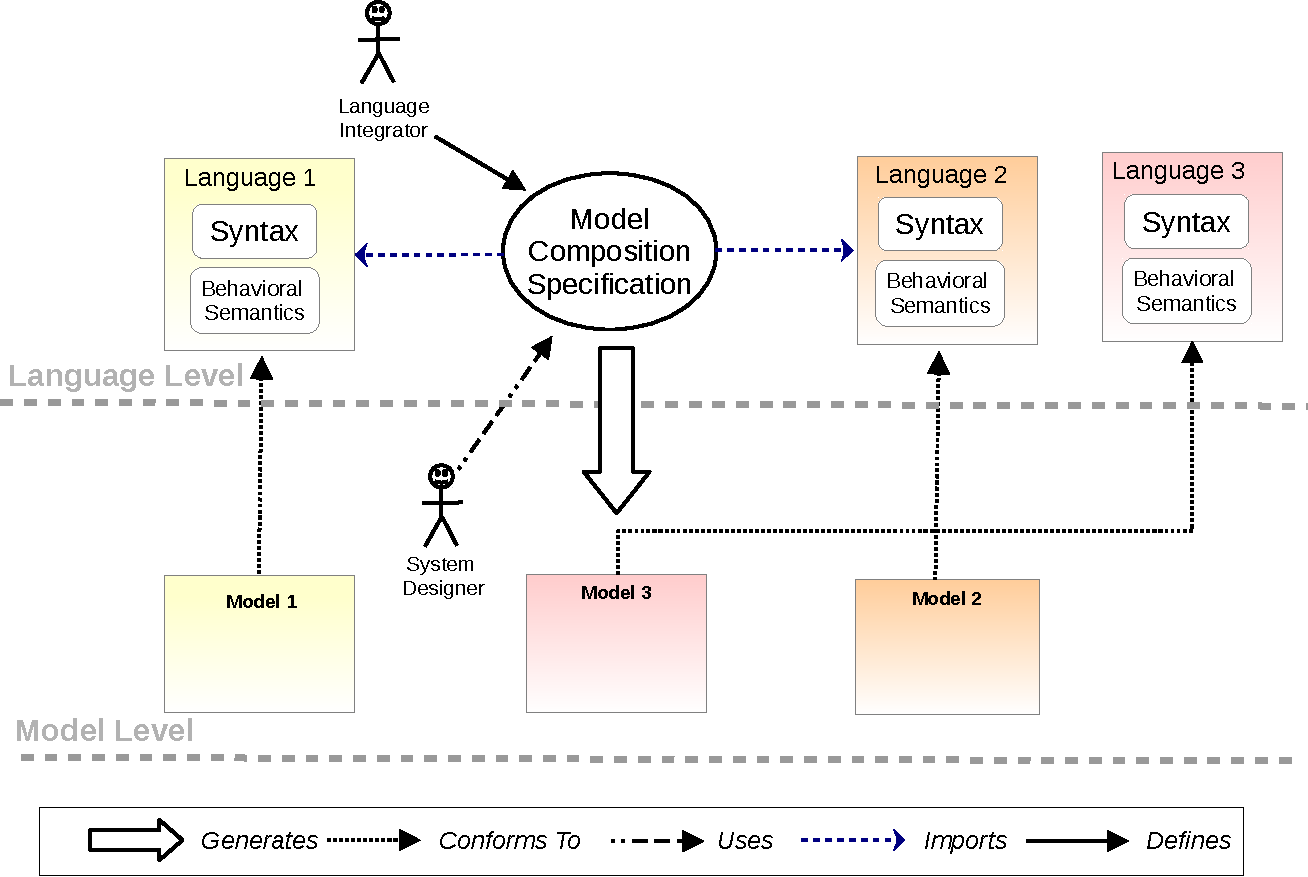
\includegraphics[width=1\textwidth]{background/figs/modelcompo}
		\caption{Model Composition Approaches Sketching}
		\label{fig:modelcompo}
	\end{center}
\end{figure}

Some approaches~\cite{mergemanifest,epsilon,kompose} have automated the composition between models by expressing the composition with two operators: \emph{matching} and \emph{merging}. The matching operator is used to look for syntactic similarities between models. This results in a set of correspondences between model elements that defines \emph{what} elements must be composed (definition in intention). From a set of correspondences, the merging operator generates a new model in which the matched elements are composed into new model elements. In~\cite{mergemanifest}, authors identified that the composition between models always relies on a merging of structure. They rely on a matching and merging operators to compare different approaches of model composition. However, they do not propose any implementation.

In~\cite{kompose}, the composition of models is also automated by relying on a matching and a merging operator. Authors proposed two generic operators: 
	\begin{itemize}
		\item A matching operator that selects model elements by comparing the signature of the elements;
		\item A merging operator that composes the selected elements by using a generic algorithm~\cite{signaturecomposebib}.
	\end{itemize}
These operators have been implemented in a tool named Kompose which is based on the metametamodel Ecore. Thus, the operators can be used to compose models that conform to different metamodels, but they conform to the same metametamodel (\ie Ecore).

While in Kompose these operators are generic, Epsilon~\cite{epsilon}\footnote{http://www.eclipse.org/epsilon/} provides dedicated languages to define both the matching and merging. The matching is specified in the \emph{Epsilon Comparison Language} (ECL) and the merging is specified in the \emph{Epsilon Merging Language} (EML). ECL is used to define \emph{matching rules} to specify correspondences between concepts of two metamodels. Matching rules apply between models and select elements that must be composed. Then, the EML is used to define \emph{merging rules} that specify how the matched elements must be composed. This results in a new model. The metamodel of both the input models and the output models must conform to Ecore.

The approaches previously studied rely on structural similarities of the models for the composition. In other words, the matching operator only focus on the syntax of languages. While this works well with structural models such as class diagrams, it becomes a limitation when working, for instance, with Sequences Diagrams (SD). Thus, to produce a meaningful composition operators for SD, the order in which events and messages have to be composed is based on the semantics of the language. In the following, we present some approaches that have addressed this problem by proposing an asymmetric composition of models. 

Aspect Oriented Modeling approaches (AOM)~\cite{sequenceweavingbib,rambib,composdbib} propose an asymmetric composition of models in which one model plays the role of \emph{base} and other the role of \emph{aspects}, both models conform to the same language. The composition of aspects into the base model is named \emph{weaving}. An aspect is made of a \emph{pointcut} and an \emph{advice}. The pointcut is a predicate over a model that is used to select relevant model elements called \emph{join points}. The join points are correspondences between the aspects and the base model. During the weaving, the join point are matched in the base model, and then, they are replaced by the advice, \ie the elements of a model (aspects), conform to a metamodel, are injected (woven) to another model that conforms to the same metamodel. The weaving acts as merging operator that replaces the join points by the advice. 

In some approaches, the weaving of aspects considers the behavioral semantics of languages. For example, in~\cite{rambib}, authors propose the weaving of aspects in which the base model and the aspects are represented by SD. An aspect is defined as a pair of SD: one SD serves as a pointcut (specification of the behavior to detect), and one serves as an advice (representing the expected behavior at the join point). When a behavior in the base model is detected, the join point is replaced by the SD that represents the advice. However, the detection of behaviors cannot be performed by only considering the syntax of the SD~\cite{problemsweavebib}. For example, consider a loop over a basic scenario where we have a message `a' and then a message `b'. We want to weave some extra-behaviour into our system each time a message `a' directly follows a message `b'. The only way to detect such a behavior is to unroll the loop thus using knowledge about the semantics of the loop construct. Therefore, these approaches use the knowledge of the behavioral semantics of languages for the weaving. However, the weaving algorithm varies depending on the approach. Thus, the resulting SD varies from one approach to other.

In this subsection, we have presented approaches that automated the composition between models by relying either on a matching and merging operator or a weaving of aspects. Most of these approaches focus on the syntax of languages. Some of them have identified that, in some cases, is necessary information about the behavioral semantics of the languages to compose the models. These approaches support the heterogeneous modeling of a system by providing composition capabilities. In this context, they seem suitable for development of a single system by using different DSMLs. In the next subsection, we present approaches that propose to compose languages into a new language.

\subsection{Language Composition Approaches}
Language composition approaches provide techniques to compose languages into a new language (see Figure~\ref{fig:langcompo}). We begin by presenting approaches that compose the syntax of languages into a new syntax~\cite{metamodelcompo}. Then, we present an approach~\cite{semanticsanchoring} that proposes to define the behavioral semantics of a language as the composition of different language behavioral semantics. 

\begin{figure}
	\begin{center}
		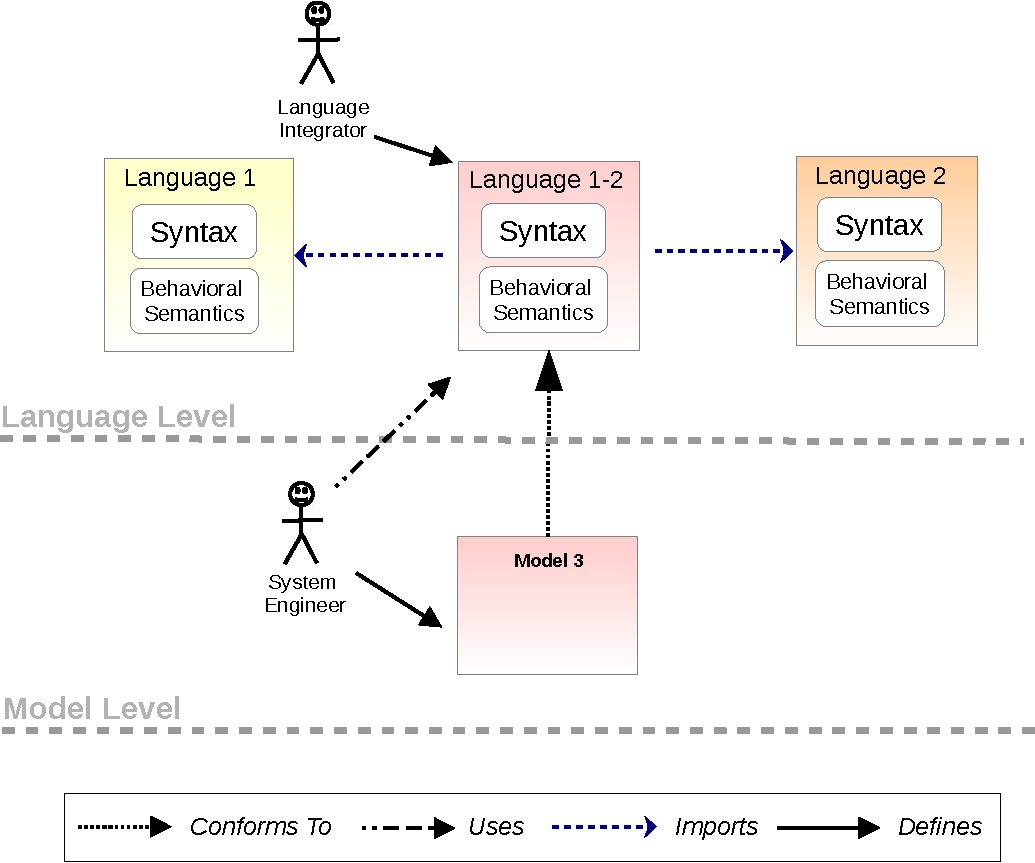
\includegraphics[width=.7\textwidth]{background/figs/langcompo}
		\caption{Language Composition Approaches sketching}
		\label{fig:langcompo}
	\end{center}
\end{figure}

In the literature, several techniques exist that compose the syntax of different languages into a new language syntax. For example, Emerson et al.~\cite{metamodelcompo} propose three of them:
\begin{itemize}
	\item \textbf{Merge:} The merging composes two languages that share a concept. These concepts are used as ``join points" to stitch the two languages together into a unified whole;
	\item \textbf{Interfacing:} When languages do not present join points, the composition requires an interface. Thus interfacing composes languages that capture distinct but related domains by relying on an interface;
	\item \textbf{Refinement:} One language captures in detail a modeling concept that exists only as a ``blackbox" in a second DSML, \ie the concept defined in one language refines in other in the second language.
\end{itemize}
These techniques have been implemented in the GME framework~\cite{metamodelcompo}, which is based on the metametamodel MetaGME\footnote{http://w3.isis.vanderbilt.edu/projects/gme/meta.html}. The refinement and interfacing have also been implemented in Monticore~\cite{monticore}. In this approach, these techniques are named: \emph{inheritance} and \emph{language embedding}. A different approach is Neverlang~\cite{neverlang} that relies on interfacing to build a custom language from features coming from different General Purpose Languages. A feature, such as the syntactical aspect of a loop, is encapsulated in a \emph{module block}. The blocks can be composed together for generating the compiler/interpreter of the resulting language. 

\emph{Semantic Anchoring}~\cite{semanticsanchoring} proposes to define the behavioral semantics of a language by relying on the concept of \emph{Semantic Unit} (SU). A SU is itself a language identified as ``basic", \eg Finite State Machine (FSM), Timed Automaton (TA) and Hybrid Automaton (HA). A SU is defined as a AsmL\footnote{http://research.microsoft.com/en-us/projects/asml/} specification in terms of (a) an AsmL Abstract Data Model (which corresponds to the abstract syntax), (b) the behavioral semantics (which is defined by the ASM mathematical framework).  SUs can be composed into a new SU. Roughly speaking, the composition is expressed manually by using AsmL. 

The approaches proposes to define a DSML by:
\begin{itemize}
	\item Defining the syntax by its metamodel; 
	\item Defining the behavioral semantics by specifying the model transformation rules between the metamodel of the DSML and the abstract data model of a SU.   
\end{itemize}
Such a SU could be the result of the composition of other SUs. For example, in~\cite{composemanticanch}, a SU named FSM (Finite State Machine) and a SU named SDF (Synchronous Data Flow) are composed to get a new SU called SU-EFSM. Then, this SU can be used to define the behavioral semantics of a heterogeneous DSMLs.

In this subsection, we presented approaches that proposed to compose the syntax and the behavioral semantics of languages into a new language syntax and behavioral semantics. These approaches proposed to model a heterogeneous system by using a single language which results from the composition of different languages. In this next subsection, we discuss about the reviewed approaches.

\subsection{Discussion}
In this section, we presented approaches that have addressed the problem of the use of heterogeneous DSMLs by providing composition capabilities between model/languages.

Model composition approaches automate the composition between heterogeneous models by relying on matching and merging operators~\cite{mergemanifest,epsilon,kompose}. In particular, Epsilon~\cite{epsilon} eases the customization of operators by providing dedicated languages. Thus, the specification of the composition can be adapted as needed. In these approaches, input and output models can conform to different metamodels, but they must conform to the same metametamodel. Most of these approach considers only the syntax of languages thus ignoring their semantics. Only a few approaches consider the semantics of languages for the composition~\cite{sequenceweavingbib,rambib,composdbib}. However, they only compose homogeneous models, \ie sequence diagrams~\cite{rambib}. Furthermore, in these approaches, the composition is encoded inside a tool. Then, to modify the specification of the composition, it is necessary to modify the implementation itself thus limiting the customization. 

Languages composition approaches propose to model heterogeneous system by relying on a unified language. Such a language results from the composition of different languages. The presented techniques~\cite{metamodelcompo} focus on the composition of syntaxes into a new language syntax. Only semantic anchoring~\cite{semanticsanchoring} enables the definition of the behavioral semantics of a language by composing other behavioral semantics through the notion of Semantics Units. Authors state that its solution is to define semantics for heterogeneous DSMLs as the composition of semantic units. However, the developing of heterogeneous systems may involve different domain experts that use different languages. In this context, this approach does not seem suitable for separation of preoccupation and development of a single system by various domain experts.

We present in the next section a different kind of approaches that propose to \emph{coordinate} heterogeneous models/languages. 


%\subsection{Overview}
%Model composition is a modeling approach used in software engineering to combine models with a specific purpose. Clavreul~\cite{clavreulmodelcompo} defines model composition as the activity that ``\textit{enables to build a system from the union of independent or dependent software artifacts}''. A model is built based on a language described by its meta model. A metamodel is a model that is developed by using a meta meta language, \eg MOF, ECORE. A metamodel defines the concepts and relations allowed in a model.

%Model composition proposes to specify \emph{correspondences} between the elements of the models (or meta-models) to be combined. Clavreul also identifies various \emph{interpretations} to these correspondences. An interpretation defines how the concepts are combined into a new model/language element. We rely on this vocabulary to analyze the state-of-art approaches. We categorize them into approaches that compose models and approaches that compose meta models. We name the former \emph{Composition of Model Approaches} and the latter \emph{Composition of Languages Approaches}.    

%Composition of model approaches have as goal to get a resulting model that is built by combining one or more models of the same language or from different languages. The resulting model can conform to input models or to a different metamodel. In~\cite{mergemanifest} the composition between two models always relies on a \emph{merging} of structures. The merging is associated with an operator that takes two models as input and applies a \emph{relationship}. The relationship contains correspondences between model elements, each correspondence defines \emph{what} elements must be composed. This approach proposes to automate the generation of correspondences by relying on a \emph{matching} operator that looks for syntactic similarities between models. From a set of correspondences, the merge operator generates a new model in which the matched elements are composed into a new element. In this work, authors suppose input and output models conform to the same language, however, they conclude that the framework could be extended to the heterogeneous case. By relying on this framework, authors have achieved to compare different approaches of model composition. However, they do not propose an implementation. 

%In Kompose~\cite{kompose} the composition of models is automated by relying on \emph{matching} and \emph{merging} operators. The matching operator specifies which concepts from different languages are related. The merging operator specifies how the matched elements are combined. The approach enables the system designer to specialize the operators to a meta metamodel. For example, the tool named Kompose is based on the meta metamodel Ecore. Thus, the operators compose models that conform to different metamodels, but they conform to the same meta metamodel (\ie Ecore).

%To ease the task of defining these operators, Epsilon~\cite{epsilon}\footnote{http://www.eclipse.org/epsilon/} provides dedicated languages to define both the matching and merging. The matching is specified in the \emph{Epsilon Comparison Language} (ECL) and the merging is specified in the \emph{Epsilon Merging Language} (EML). The ECL is used to define \emph{matching rules} that enable the developer to specify correspondences between concepts of two metamodels. Matching rules apply between models and select elements that must be combined. Then, the EML is used to define \emph{merging rules} that specify how the matched elements must be combined. This results in a new model. The metamodel of both the input models and the output models must conform to Ecore.

%\todo{To explain that the comparison is only between classes}

%\todo{To illustrate by using a Epsilon Specification}

%The approaches previously studied only rely on structural similarities of the models to compose. While this works well with structural models such as class diagrams, it becomes a limitation when working with sequence diagrams. To produce a meaningful composition operator for sequence diagrams, the order in which events and messages have to be composed is based on the semantics of sequence diagrams. Thus, other approaches have focused on establishing semantic correspondences between models. They also rely on matching and merging operators, but they consider both structural and semantic information in the models.  

%The principal limitation of the proposed approach is that to be reusable the framework only relies on the structure of the models to compose. The signatures are the only elements which can be used to take into account some semantics of models to compose. Our current experiments show that it is not an issue when working with structural models such as class diagrams, database schemas or components model but it becomes a clear limitation when working with modelling languages such as sequence diagrams. 

%Nejati et. al~\cite{compostatechartsbib} propose to represent the behavior of models by using statecharts. They propose an automatic approach to compose statecharts into a new statechart that represent the resulting behavior. The approach is based on matching and merging operators. These operators rely on both structural and semantic information in the models. The matching operator is made of a combination of a \emph{static matching} and a \emph{behavioral matching}. The static matching identifies correspondence relationships between states by relying on their names. Thus, it is independent of the semantics of statechart and it is not different that the correspondence presented in the previous approaches. Conversely, the behavioral matching identifies correspondence relationships between states by relying on their behavior. For instance, the approach relies on measuring how close the behavior of one state is to that of another. To do so, they compute a similarity degree for every pair of states by comparing the immediate neighbors of each pair of states. In this approach, a neighbor is either a successor/child state (forward neighbor) or a predecessor/parent state (backward neighbor). By relying on a static and behavioral matching, the matching operator returns a set of correspondences between states. Then, the merge operator takes as input two statecharts and the correspondences, and generates as output another statechart model.
       
%Aspect-Oriented Modeling approaches~\cite{weavingbib} also consider the dynamic properties of models for the composition. However, in these approaches, the mechanism used to compose models is different. One model plays the role of \emph{base} and other the role of \emph{aspect}, both models conform to the same language. The composition of aspects into the base model is called \emph{weaving}. An aspect is made of a \emph{pointcut} and an \emph{advice}. The pointcut is a predicate over a model that is used to select relevant model elements called \emph{join points}. The join points are correspondences between the aspect and the base model. During the weaving, the join points are replaced by the advice, \ie the elements of a model (aspects), conforming to a meta-model, are injected (woven) into another model that conforms to the same meta-model. In some approaches, the weaving of aspects is done by considering the behavior of the models used. For example, in~\cite{sequenceweavingbib,rambib,composdbib}, the behavior of a model is represented by a Sequence Diagram (base model). An aspect is defined as a pair of SD: one SD serves as a pointcut (specification of the behavior to detect), and one serves as an advice (representing the expected behavior at the join point). When a behavior in the base model is detected, the join point is replaced by the SD that represents the advice. The algorithm used for the weaving may vary from one approach to another thus resulting in a different SD depending on the approach. 

%\todo{To illustrate by showing un example of weaving}

%The previous approaches manage the composition of models in order to generate a new model. Conversely, composition of language approaches compose languages in order to generate a new language. In these latter approaches, the correspondences associate concepts of various metamodels in order to generate a new metamodel. The composition is done by a system designer that specifies \emph{what} and \emph{how} concepts from different metamodels are related. In the literature, several techniques exist that compose the structure of languages into a new language. For example, Emerson et al.~\cite{metamodelcompo} propose three of them:
%\begin{itemize}
%	\item \textbf{Merge:} It is used to compose two languages that share a concept. These concepts are used as ``join points" to stitch the two languages together into a unified whole;
%	\item \textbf{Interfacing:} When languages do not present joint points, the composition requires an interface. Thus interfacing composes languages that capture distinct but related domains by relying on an interface;
%	\item \textbf{Refinement:} One language captures in detail a modeling concept that exists only as a ``blackbox" in a second DSML, \ie the concept defined in one language is refined in the second language.
%\end{itemize} 
%These techniques enable the composition of different languages by relying on the same meta meta model. For example, these techniques have been implemented in the GME framework~\cite{metamodelcompo}, which is based on the meta meta model MetaGME\footnote{http://w3.isis.vanderbilt.edu/projects/gme/meta.html}. Many other approaches present variation of these techniques. For instance, Monticore~\cite{monticore} propose two techniques: \emph{inheritance} and \emph{language embedding}. These techniques correspond respectively to refinement and interfacing. A different approach is Neverlang~\cite{neverlang} that enables to build a custom language from features coming from different General Purpose Languages. A feature, such as the syntactical aspect of a loop, is encapsulated in a \emph{module block}. The blocks can be composed together for generating the compiler/interpreter of the resulting language. This approach can be understood as an ``interfacing" between general purpose programming languages.

%These techniques only provide the means to compose the structure of languages. However, they make explicit neither the semantics of the language nor the semantics of the composition. Differently, \emph{Semantic Anchoring}~\cite{semanticsanchoring} proposes to explicitly define the behavior semantics of a language. Furthermore, it enables the definition of how the semantics can be composed to obtain a new semantics. To describe the behavioral semantics of a language, the approach relies on the concept of \emph{Semantic Unit} (SU). A SU is itself a language identified as ``basic", \eg Finite State Machine (FSM), Timed Automaton (TA) and Hybrid Automaton (HA). A SU is defined as a AsmL\footnote{http://research.microsoft.com/en-us/projects/asml/} specification in terms of (a) an AsmL Abstract Data Model (which corresponds to the abstract syntax), (b) the behavioral semantics (which is defined by the ASM mathematical framework). Then, the approach proposes to:
%\begin{itemize}
%	\item Define the syntax of a DSML by its metamodel;
%	\item Define the behavioral semantics of a DSML by specifying the model transformation rules between the metamodel of the DSML and the Abstract Data Model of a semantic unit. 
%\end{itemize}    
%The main benefit of the use of SUs is that they can be composed into a new SU. For example, in~\cite{composemanticanch}, a SU named FSM (Finite State Machine) and a SU named SDF (Synchronous Data Flow) are composed to get a new SU called SU-EFSM. Roughly speaking, the composition is expressed manually using AsmL. Then, the resulting SU can be used to define the behavioral semantics of a language.

%\subsection{Discussion}
%Composition of Model approaches automate the composition between models by relying on a matching and merging operators. Furthermore, Epsilon eases the customization of operators by dedicated languages. The system designer can adapt the composition as needed. In these approaches, input and output models can conform to different metamodels, but they must conform to the same meta metamodel. However, these approaches can only specify the composition between two languages thus limiting its usage for heterogeneous systems. Besides, they only consider structural models thus ignoring their semantics.     

%In~\cite{compostatechartsbib,weavingbib}, approaches have automated the composition of models by considering both syntactic and behavioral similarities. However, in these approaches, the composition is always specified between homogeneous models. Furthermore, operators are encoded inside a framework thus limiting the tuning of the specification. In addition, the detection of behavioral similarities between models is not easy or sometimes impossible as shown in~\cite{?}. 

%Composition of Languages propose to model heterogeneous systems by relying on a unified language. Such a language results from the composition of other languages. Unlike the composition of models, the composition of languages have not been automatized. Instead, a system designer has to 1) find correspondences between concepts of different languages and 2) specify how these concepts are related. This activity results in a new language. The input languages and the composed language conform to the same meta metamodel. In most of these approaches, correspondences are only between syntactic elements, and only one enables to define behavioral correspondences in order to obtain a new behavioral semantics. In this latter approach, authors state that its solution is to define semantics for heterogeneous DSMLs as the composition of semantic units. However, these approaches do not seem suitable for separation of preoccupation and development of a single system by various domain experts. 
